%%%%%%%%%%%%%%%%%%%%%%%%%%%%%%%%%%%%%%%%
% Class options                        %
%%%%%%%%%%%%%%%%%%%%%%%%%%%%%%%%%%%%%%%%
% Orientation:                         %
% portrait (default), landscape        %
%                                      %
% Paper size:                          %
% a0paper (default), a1paper, a2paper, %
% a3paper, a4paper, a5paper, a6paper   %
%                                      %
% Language:                            %
% english (default), norsk             %
%%%%%%%%%%%%%%%%%%%%%%%%%%%%%%%%%%%%%%%%
\documentclass[landscape]{uioposter}


\usepackage{lipsum}              % Dummy text
\usepackage{graphicx}
\usepackage{listings}
\usepackage{color}
\usepackage[figwidth=0.98\linewidth]{todonotes}  % Dummy image (and more!)
\usepackage[absolute, overlay]{textpos}            % Figure placement
\setlength{\TPHorizModule}{\paperwidth}
\setlength{\TPVertModule}{\paperheight}


\title{An Interactive Web-based GIS System to Evaluate Hurricane Inundation Impacts}
\author
{%
    Michael Bednarek%\inst{1}
    \and
    Saeed Moghimi%\inst{2}
}
%% Optional:
%\institute
%{
%    \inst{1} Department of Mathematics
%    \and
%    \inst{2} Department of Informatics
%}
%% Or:
%\institute{Contact information}


%% Remove footline:
%\setbeamertemplate{footline}{}


\begin{document}
\begin{frame}
\begin{columns}[onlytextwidth]


\begin{column}{\textwidth/3 - 2cm}
    \begin{block}{Introduction}
        The 
    \end{block}

    \begin{block}{Collection}
        Ramble here about where we get the data.
        - NetCDF
        - Models
    \end{block}
    
    \begin{block}{Processing}
        Discuss contouring and formatting.
        In order to more easily interact and manipulate the data, it is first formatted and contoured. A collection of polygons is read from the NetCDF file which is to be converted into a more accessible format.
        For this project the format of choice is JSON as it easy to manipulate in a multitude of languages and protocols while still supporting all necessary features.
        
        The NetCDF file contains only a raster of points and according elevation values.
        For both space saving and ease of manipulation, these values are grouped and vectorized to a collection of polygons.
        A given amount of levels is given in which a polygon may exist. A smaller level count indicates larger but fewer polygons, making a lower resolution but smaller file.
        These polygons are then encoded into a JSON file including some general information about it's size, value, and resolution.
        
        The format of a contoured cache:
        
        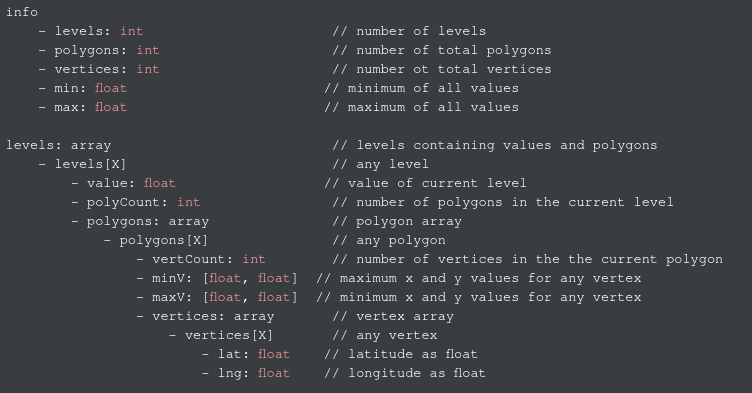
\includegraphics[scale=0.6725]{screenshot1.png}

    \end{block}
    
\end{column}


\begin{column}{\textwidth/3 - 2cm}
    \begin{block}{Serving}
        Talk about protocol and API functionality.
        A Flask web server is used to serve the compressed information created from the processing phase.
        Flask is the library of choice here as it requires little boilerplate code to function however it still retains the functionality and documentation of other solutions.
        Written in Python, it is easy to integrate with existing functions and libraries.
        The server provides the computations and implementation for a number of methods of interacting with the collected data.
        This includes transection, regional mapping, and a number of methods for interpreting the compressed polygons.
        Originally written manually, the primary methods for interaction and calculations with polygons are done using the Shapely library.
    \end{block}

    \begin{exampleblock}{Interface}
        Talk about handling of an example such as Sandy.
        Show images including polygons and GUI.
        
        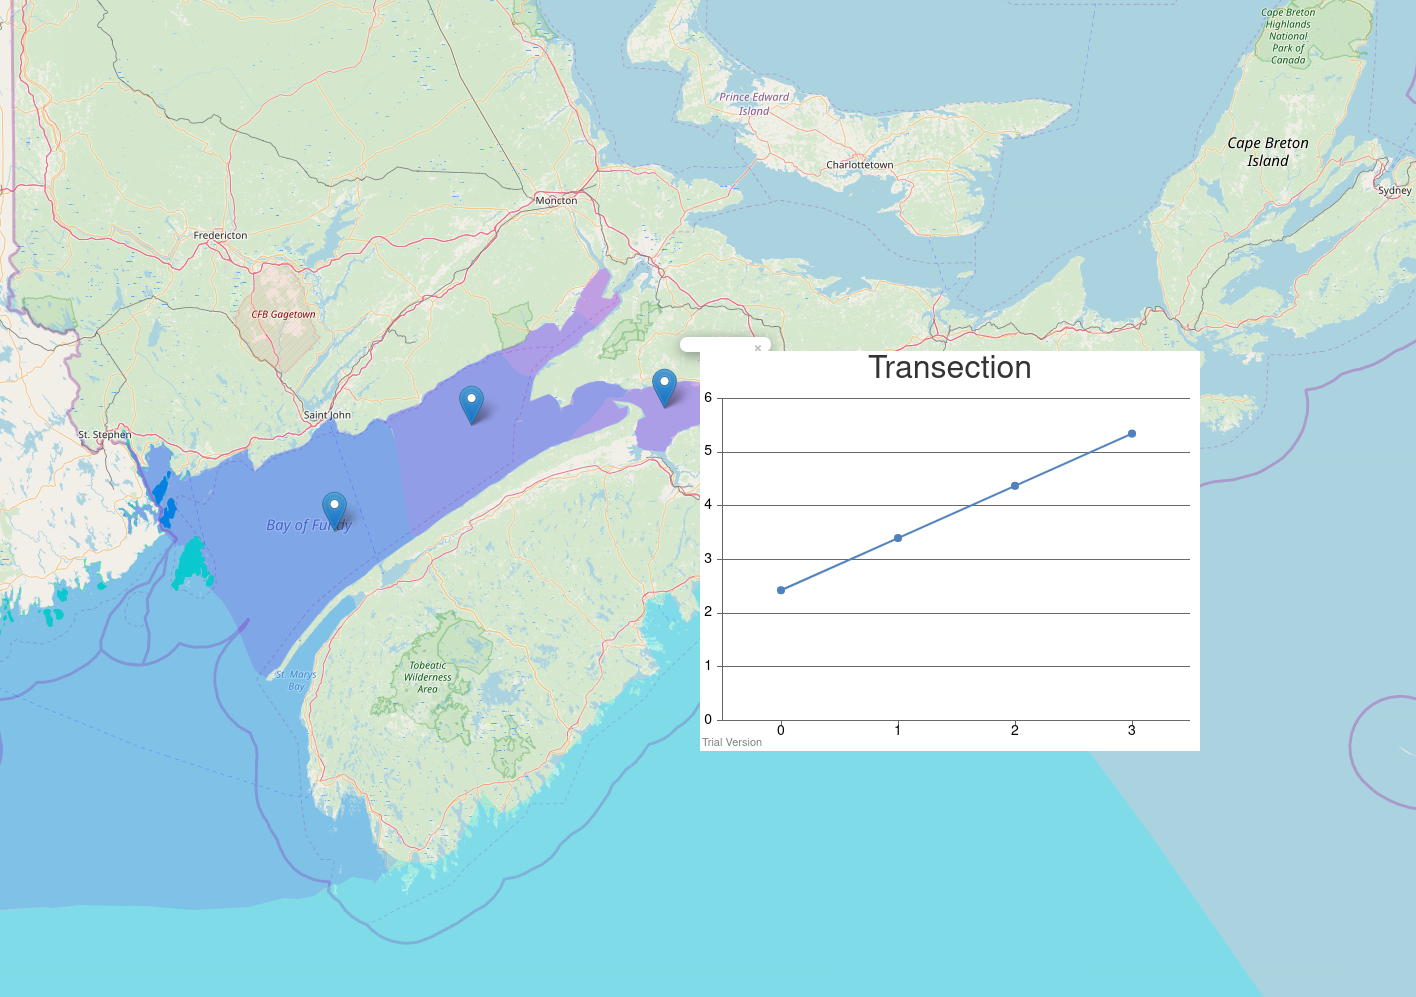
\includegraphics[scale=0.6725]{screenshot.png}
        
    \end{exampleblock}
\end{column}


\begin{column}{\textwidth/3 - 2cm}
    \begin{block}{Purpose}
        Talk about purpose behind project and possible uses.
    \end{block}
    
     \begin{block}{Process}
        Talk about development process.
    \end{block}
    

    \begin{block}{Improvements}
        Talk about possible future improvements for the project.
    \end{block}
\end{column}


\end{columns}


\begin{textblock}{0.5}(0.025, 0.9575)
    \color{white}
    \sffamily
    \textbf{Github Organization}
    \\
    https://github.com/earth-sys-ai
\end{textblock}


\end{frame}
\end{document}